\documentclass[border=2pt]{standalone}
\usepackage{pgfplots}
\usepackage{amsmath}
\begin{document}
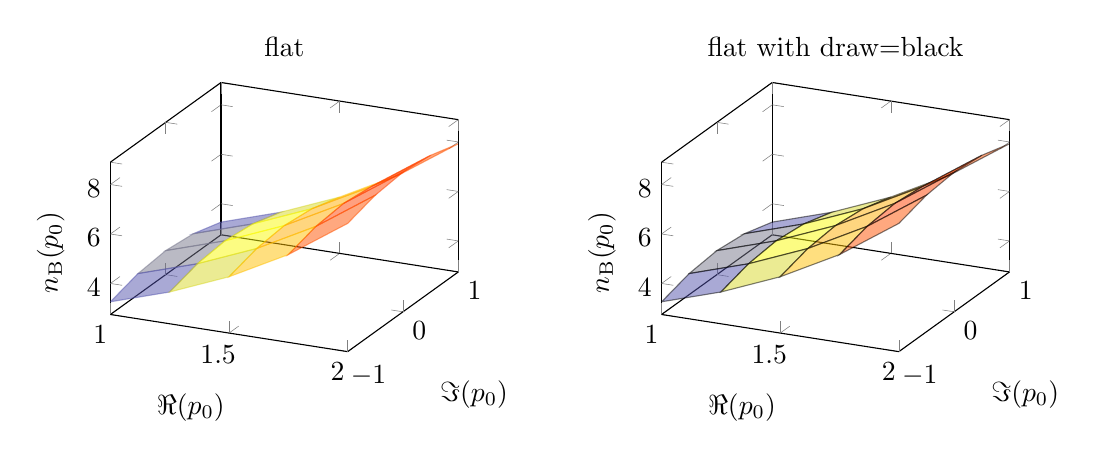
\begin{tikzpicture}
\begin{axis}[width=6cm,height=5cm,shader=flat,title={flat},
  xlabel=$\Re(p_0)$,ylabel=$\Im(p_0)$,zlabel=$n_\text{B}(p_0)$]
  \addplot3[surf,opacity=0.5,domain=1:2,y domain=-1:1,samples=5]
    {e^x + cos(deg(y))};
\end{axis}
\begin{axis}[at={(7cm,0)},width=6cm,height=5cm,shader=flat,title={flat with draw=black},
  xlabel=$\Re(p_0)$,ylabel=$\Im(p_0)$,zlabel=$n_\text{B}(p_0)$]
  \addplot3[surf,draw=black,opacity=0.5,domain=1:2,y domain=-1:1,samples=5]
    {e^x + cos(deg(y))};
\end{axis}
\end{tikzpicture}
\end{document}
